\chapter{Background}
In this section, we give background on the different concepts and technologies used in this thesis, which include logic-based reasoning Simulink, stochastic timed automata,  statistical model checking, integer-linear programming and population-based metaheuristics.
\section{Logic-based Reasoning}
In this thesis, we express requirements specifications in  Boolean logic and apply \textit{Boolean satisfiability} (SAT) to detect inconsistencies within the specifications. Furthermore, we use \textit{ontology} to represent the specifications, and conduct rigorous analysis via a linguistic approach.
\subsection*{Boolean Satisfiability}
The study of a Boolean formula is generally concerned with the set of truth assignments (assignments of 0 or 1 to each of the variables) that make the formula true. Finding such assignments by answering the simpler question: ``does there exist a truth assignment that satisfies the Boolean formula?'' is called the Boolean satisfiability problem (SAT), which is proven to be NP complete~\cite{devlin2008satisfiability}\cite{Biere2009HandbookSatisfiability}. However, efficient heuristics and approximation algorithms do exist to solve such problems.

SAT problems are usually checked using decision procedures known as SAT solvers. Z3 integrates several background theories (or Satisfiability Module Theories, SMT) and decision procedures based on SAT solvers~\cite{DeMoura2008Z3:Solver}. It is a well known SMT solver and a theorem prover developed by Microsoft Research which has been used in the formal verification and reasoning of software and hardware systems, mainly due to its strong support for integration to verification tools via its well known APIs written, e.g., in Java, Python, C.

Z3's input language is an extension of the SMT-LIB2 standard, which are commands used to assert logical statements and instruct the solver to do some action, e.g., to check for satisfiability, the command \textit{(check-sat) }is invoked. Z3 returns \textit{sat} if the formulas are satisfiable. If the formulas are not satisfiable, Z3 returns \textit{unsat}, or if it cannot decide the result, it returns \textit{unknown}. In case of unsat, if the unsat-core option is enabled, Z3 can return the subset of unsatisfiable assertions by invoking the \textit{(get-unsat-core)} command.

\subsection*{Ontology and Description Logic}
Ontology is a knowledge representation technique frequently used in the artificial intelligence and other domains to facilitate automated decision making. It is defined as ``a formal specification of a shared conceptualization'' according to Borst \cite{Borst1997ConstructionOntologies}. It employs different modeling entities, e.g., concepts, instances, axioms, which are compared to classes, objects, inheritance in Object-Oriented Programming. The ontology is consistent if every axioms and relations (or assertions) hold~\cite{Mankovskii2009OWL:Language}.

Description logic (DL)~\cite{Baader2010TheApplications} is a knowledge presentation language, and is the most widely language used to construct ontologies. It is a fragment of first-order logic with many of the core reasoning problems decidable. For this reason, it has several application, e.g., in web semantics (e.g., OWL)~\cite{conf/owled/ShearerMH08}, artificial intelligence~\cite{10.1007/978-94-017-9297-4_7}, bioinformatics~\cite{Rector2006}, software engineering, natural language processing. Thus, it is usually backed by solid reasoning services that terminate and deliver results in reasonable time. 

\section{Simulink}
Simulink~\cite{JamesB.Dabney2003MasteringSimulink} is a graphical development environment for the modeling, simulation and analysis of embedded systems which is widely used in industry to model and inspect the dynamics of systems before implementation. It is robust as it supports multi-domain, continuous, discrete, hybrid systems, also discrete systems that execute with different sampling times (or multi-rate). Figure~\ref{fig_sm_multi-rate} shows a multi-rate subsystem of the brake-by-wire Simulink model that models the brake pedal (i.e., continuous behavior) and global brake functionality (i.e., discrete behavior), which executes every 10ms and 20ms.  
\begin{figure}[h]
	\centering
	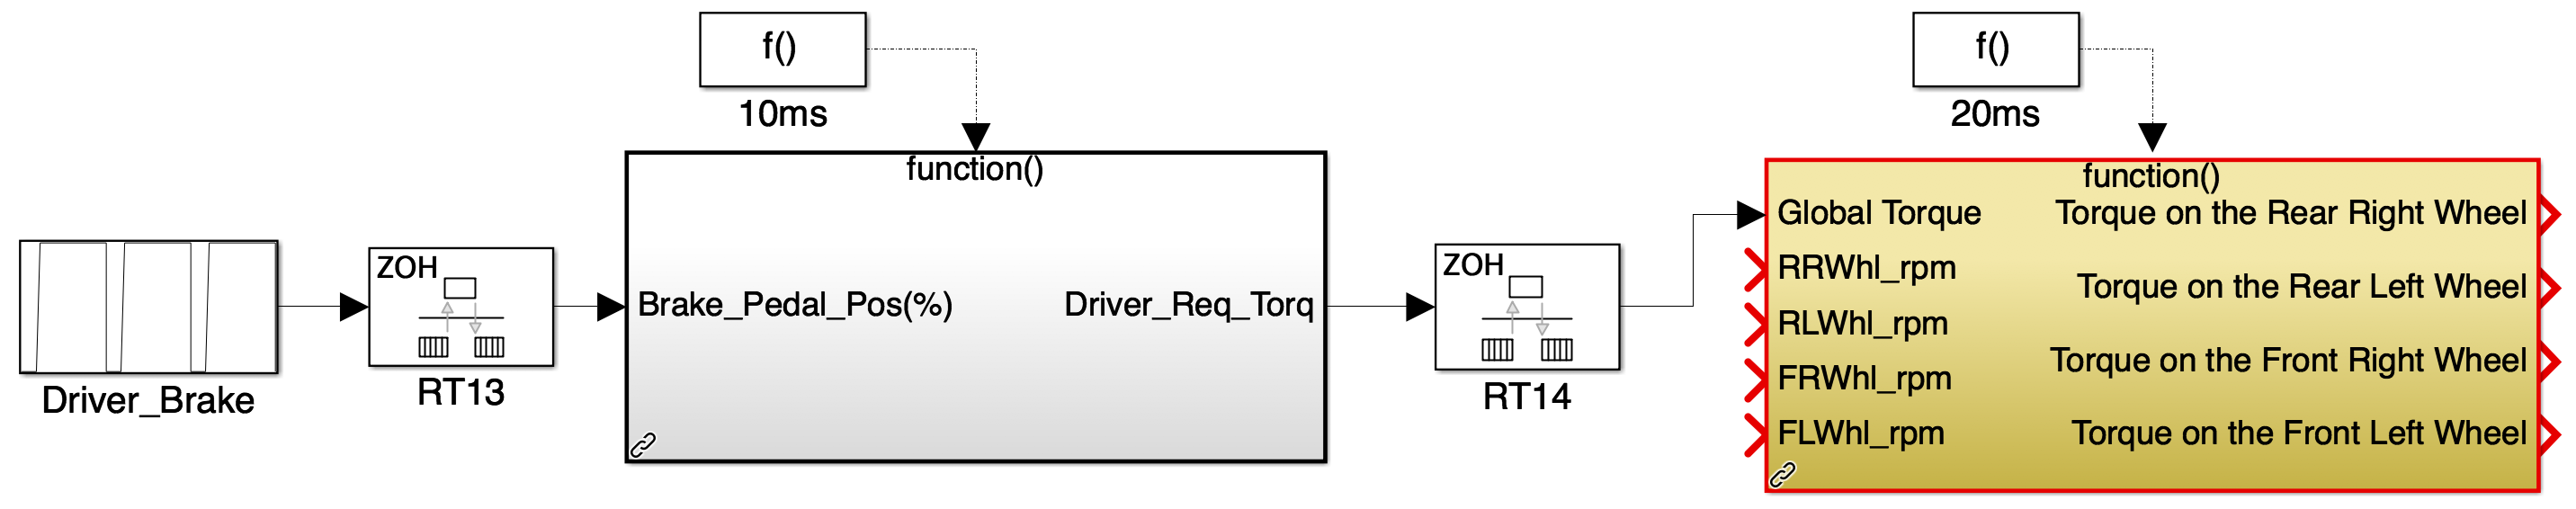
\includegraphics[width=0.9\linewidth]{images/sm}
	\caption{Brake pedal and global brake controller of the brake-by-wire model.}
	\label{fig_sm_multi-rate}
\end{figure}

Simulink is frequently used in the development of safety-critical systems, e.g., automotive, avionics, furthermore, it is used to generate code automatically from the models. Therefore, it is crucial that such models are analyzed rigorously. The Simulink Design Verifier (SDV) provides a formal verification technique that is based on the exact model checking to exhaustively verify functional properties~\cite{MathWokrksSimulinkVerifier}, however, its functionality is limited as it lacks support for timed analysis, which is vital to ensure predictability of safety-critical embedded systems. 

\subsection*{Simulink Blocks}
A Simulink model is constructed from communicating function blocks (or Simulink blocks). The blocks implement simple to complex functionality and consist of Input and Output ports, which enable communication via connectors. The latter modeling elements support basic and user-defined datatypes, e.g., integer, floating-point; and simple and complex data structures, e.g., scalar, vector, matrix.  Simulink blocks are classified into \textit{virtual} (non-computational, e.g., Mux, Demux blocks) and \textit{non-virtual} (computational, e.g., Gain, Integrator) blocks based on their computability. The non-virtual blocks improve the visualization of the model, but unlike the non-virtual blocks, they are not executed, hence do not affect the execution semantics of the model.  The blocks can be composed into groups, e.g., using Subsystem, Model blocks, to enable hierarchical modeling, which is used to improve the visualization, and to enforce execution order on a group of blocks. The fundamental constructs of the composite blocks are \textit{atomic} blocks, e.g., Gain, Sum blocks.

The non-virtual (computational) atomic blocks can be categorized into \textit{continuous} and \textit{discrete} blocks based on the execution semantics of the blocks.  A discrete block executes periodically with sample time $t_s$, whereas a continuous block executes over infinitesimal sample times. Since the Simulink blocks libraries are not usually sufficient to model practical embedded system systems, Simulink supports mechanisms to extend functionality that engineers can exploit to develop complex systems. The mechanisms include S-function, Custom Block and Masking. S-function is a computer language of Simulink blocks which allows advanced implementations of block routines, written in MATLAB, C, C++, or Fortran.


\subsection*{Execution of Simulink Blocks}
During the initial phase of the simulation in the Simulink environment, the model is compiled, thus the order in which the blocks are executed is established in the \textit{sorted order} list. Figure~\ref{fig_sm_exec_order} shows the execution order via the labels in red color, annotated as $s:b$, where $s$ denotes the system/subsystem index and $b$ the block index\footnote{https://se.mathworks.com/help/simulink/ug/controlling-and-displaying-the-sorted-order.html}. Basically, the list is determined according to the data dependency of blocks' outputs on the blocks' input ports, i.e., if the output depends on the current value of the input, the input port is identified as \textit{direct-feedthrough} port. Thus, to preserve the data dependency in the model, the sort-order rules require that the blocks that derive other blocks with direct-feedthrough ports must come first in the list, e.g., blocks that derive Gain block. However, the blocks with non-direct-feedthrough ports, e.g., Delay block, can execute in any order, considering the previous rule applies. The execution order is also affected by the user defined priorities, nevertheless, the priorities do not violate the rules. The sorted order list can be fetched by simulating the model in the debugging mode.
\begin{figure}
	\centering
	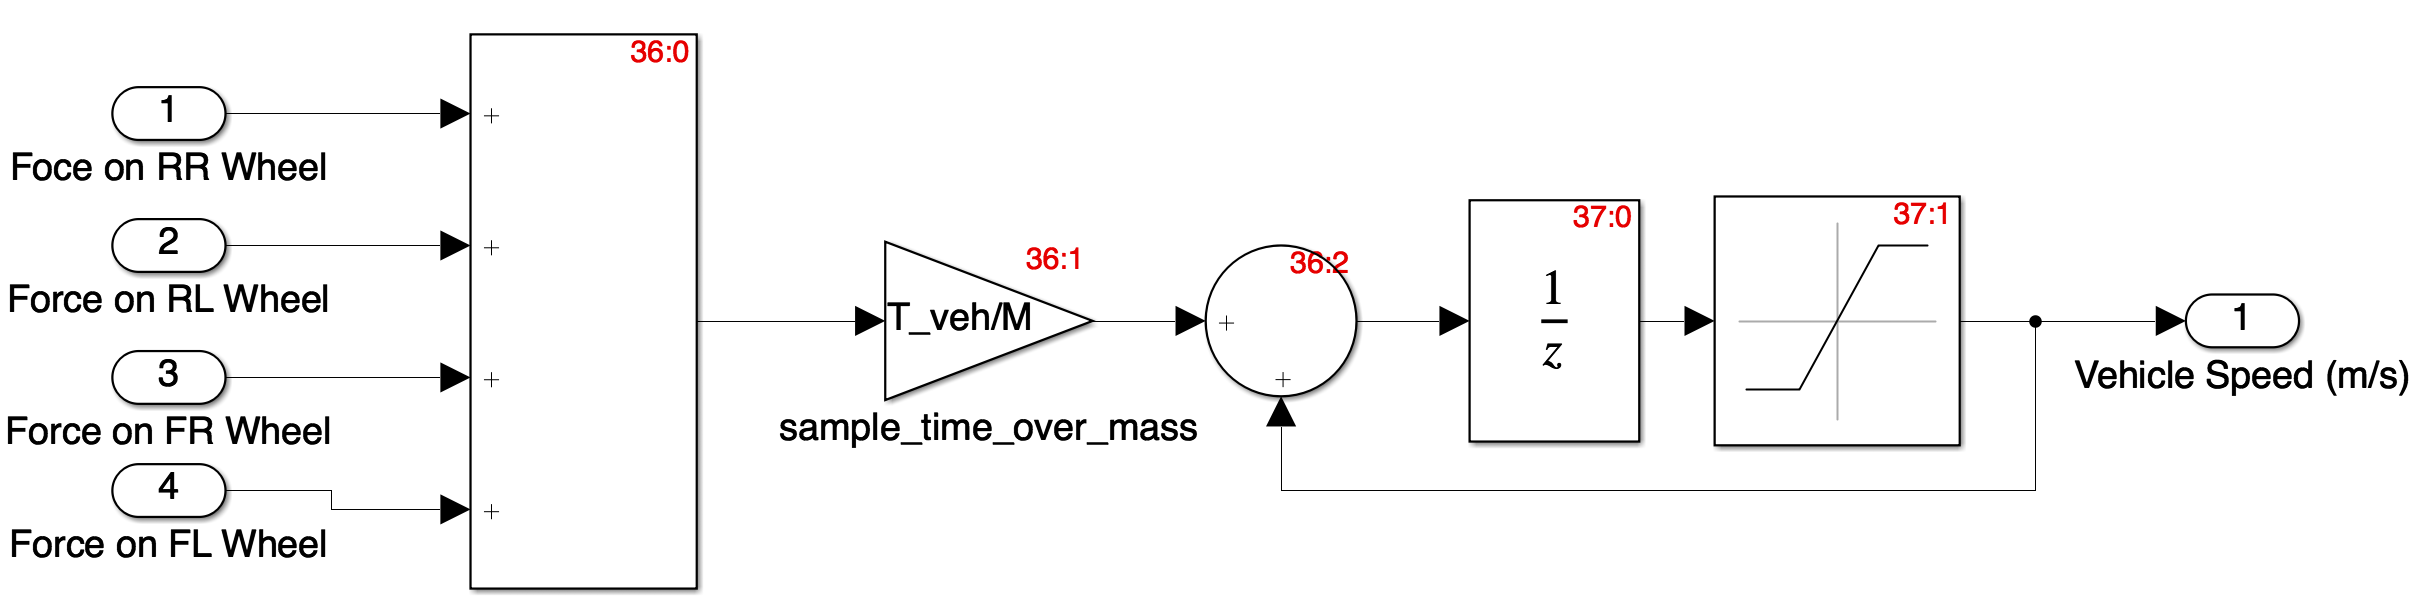
\includegraphics[width=1\linewidth]{images/sm_exec_order}
	\caption{A Subsystem block from the brake-by-wire model, computes vehicle speed. The labes in red color are indexed identifiers and denote of the execution order.}
	\label{fig_sm_exec_order}
\end{figure}

\section{Stochastic Timed Automata}
The theory of stochastic timed automata builds upon the timed automata theory via probability to support stochastic behavior in modeling and analysis of real-time systems. It can be used to model continuous-time behaviors, e.g., pressing the brake pedal, which occurs at continuous time points, and others, e.g., waiting time in network communication, uncertainly in input values, soft real-time deadlines. 

A timed automaton $\mathcal{A}$ is a finite-state automaton proposed by Alur et al.~\cite{Alur1999TimedAutomata} to model and analyze real-time systems, i.e., by extending the automaton with real-valued clock variables $X$. It is widely used in the model checking to verify functional and timing requirements, e.g.,liveness, safety properties. The stochastic version automaton $\langle\mathcal{A},\mu,\gamma\rangle$ basically extends the timed automaton with probability, i.e., on the delays between states via the delay density functions $\mu$ and discrete transitions between locations via the output probability functions $\gamma$, where  $\mathcal{A}$ is represented as a tuple $\langle L,l_0,X,\Sigma,E,I\rangle$, and its elements are described as follows: $L$ is a set of locations of which $l_0$ is the initial location, $E$ is the set of edges between locations,  $\Sigma$ is a set of action labels, and $I$ is a set of invariants, which are Boolean constraints over $X$ assigned to locations, i.e., the system (or automaton) can only stay in the location as long as its invariants hold. An edge $(l,g,a,r,l')\in E$ denotes a transition relation from the location $l$ to $l'$, with conjunctions of guards $g$, action $a$ and clock resets $r$. The guard is also a Boolean constraint over $X$, and when it holds, the transition on the edge is enabled.
\begin{figure}
	\centering
	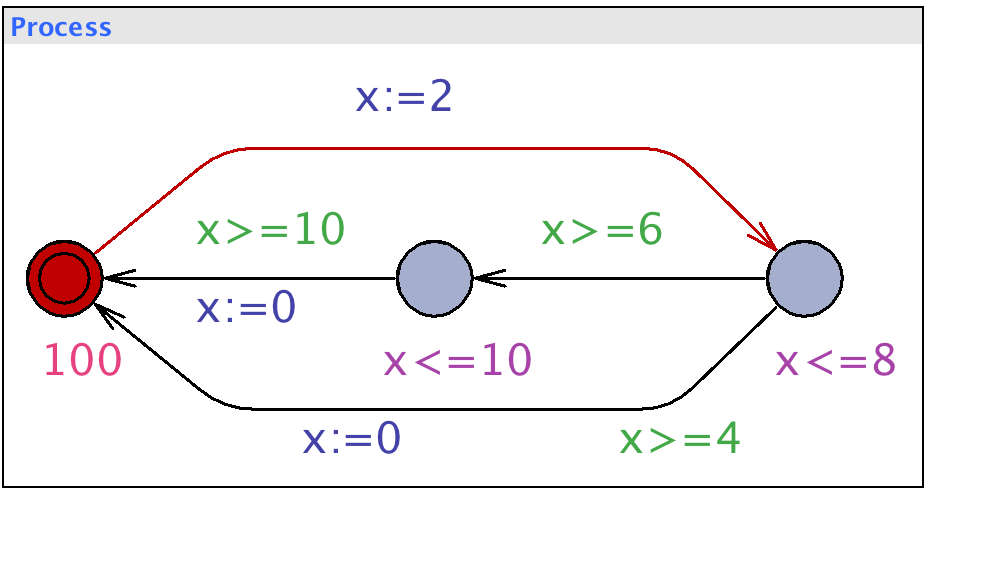
\includegraphics[width=0.6\linewidth]{images/sta_dummy_example}
	\caption{STA example.}
	\label{fig_staexample}
\end{figure}

\begin{example}[STA Example] Figure~\ref{fig_staexample} is a dummy STA example with three locations A,B and C, where A is the initial location. The guards of the automaton are labeled in Green color, the clock resets in Blue and the constraints in Red.
\end{example}

Assume that, $d(l,v)$ is the infimum delay which satisfies the disjunction of guards on the edge that start from $l$, and assume that, $D(l,v)$ is the superimum delay which satisfies the invariant $I(l)$. If the delay is bounded, i.e., there exists $D(l,v)$, in location $l$, each delay density function in $l$, $\mu_s$, is assumed to be uniformly distributed on the interval $[d(l,v),D(l,v)]$. However, if the location is time unbounded, the delays are assumed to be exponentially distributed with the rate $R(l)$. To illustrate this point, consider the same STA example, the delays at the location A are exponentially distributed, i.e., with rate 100, since the the location is time unbounded, and delays at B and C are uniformly distributed on the interval $[4,8]$ and $[10,10]$, respectively. The output probability of locations A and C is 1 and of location B is 1/2. 
%Note: logical path, and probability of taking the path is purely stochastic

\subsection*{Network of Stochastic Timed Automata}
Under the assumption of input-enabledness, disjointness of clock sets and output action sets, a network of STA (denoted by NSTA) is parallel composition of $STA_i$, i.e., $(STA||STA2||,...,||STAn)$, where n is the number of STA in the netowrk.  The state of a networked TA is a tuple $\langle s_1,s_2,...,s_n\rangle$, where $s_i=(l,v)\in L_i\times X_i$ . In NSTA, the automata communicate through broadcast channels and globally shared variables. Moreover, the semantics of the NSTA relies on the independent computation of the individual STA (or components), i.e.,  each component automaton, based on the delay density functions and the output probability functions decides repeatedly on which output to generate and at which point in time. In this race, the output will be determined by the component automaton that has chosen to produce the output after the minimum delay~\cite{David2011StatisticalAutomata}.


\section{Statistical Model Checking}
Statistical model checking~\cite{Agha2018AChecking} uses a finite set of randomly selected execution traces (or runs) of the state-based system $S$ to check if the traces provide probability evidence for accepting or rejecting the specification (or property) $\varphi$, i.e., $T\in Traces(S)\models \varphi$. It applies statistical techniques such as hypothesis testing and Monte Carlo simulation to compute the probability evidence. Since most interesting problems in timed automata, e.g., the reachability problem, become undecidable in NPTA, statistical model checking is a viable alternative to approximate the problems via probability estimation. Moreover, in contrast to the exact model checking technique, statistical model checking as any other Simulation-based techniques consumes much less memory and CPU, and returns results in much less computation time..

\uppaalsmc{} is an extension of the model checker \uppaal with support for statistical model checking. It admits a system modeled as NPTA, and the properties to checked are specified in the probabilistic extension of the WMTL (or PWMTL) logic~\cite{Bulychev2012UPPAAL-SMC:Automata}, which are expressed inductively as follows:
\begin{align}
\varphi::=P(\Diamond_{c\ C}\phi)\bowtie p | P(\Box c\leq t)\bowtie p
\end{align}
where $c$ is a clock, $C\in \mathbb{N}$ is a bound, $\phi$ is a state-predicate, $\bowtie \in\{\leq,\geq\}$, and $p \in [0, 1]$.

\uppaalsmc~\cite{David2011TimeSystems}\cite{Bulychev2012UPPAAL-SMC:Automata} can be used to check quantitative and qualitative properties via \textit{hypothesis testing} and \textit{probability comparison}, and \textit{probability evaluation}, respectively. The
hypothesis testing is a qualitative statistical method which checks if the probability of satisfying a PWMTL property is less than or equal to a certain probability threshold $p$ over a network of STA. The probability of making hypothesis testing errors is bounded by the strength parameters $\alpha$ and $\beta$, where $\alpha$ is the probability of accepting the null hypothesis while the opposite of it holds (false negative), and $\beta$ is the probability of accepting the opposite of the null hypothesis while the null hypothesis holds (false positive). Another qualitative property that can be checked using \uppaalsmc{} is the comparison of probabilities satisfying two PWMTL properties.

The probability evaluation is a quantitative method which determines the probability of satisfying a PWMTL property, $p$, over a network of NPTA. The evaluation is an approximation interval $[p-\mu,p+\mu]$ with a confidence $1-\alpha$, where $\mu$ and $\alpha$ are user configurable parameters. The number of traces are determined based on the parameters automatically by the model checker.
\vspace{2cm}
\section{Integer linear Programming}
An integer linear programming (or integer programming, \ilp) is a type of optimization problem which consists of integer decision variables, and the objective function and the constraints are linear. The binary (or 0-1) \ilp{} problem is a special case of ILP whose decision variables are binary, i.e., takes 0 or 1. It is represented as:
\begin{align}
    \label{eqn_ilp_obj}
	&Maximize\ \sum_{j=1}^{n}{c_jx_j}\\\nonumber
	\mbox{Subjec to:}&\\\nonumber
	&\sum_{j=1}^n{a_{ij}x_j}\leq b_i&\mbox{ for all } i=1,...,m\\
	&x_j\in\{0,1\} &\mbox{ for all } j=1,...,n
\end{align}
where (\ref{eqn_ilp_obj}) is the objective function with $n$ cost coefficients $c_j:j=1,...,n$, (\ref{eqn_ilp_obj}) are $m$ linear constraints with coefficients $a_j:1,...,m$ and requirements $b_j:1,...,m$, and $x_j:1,...,n$ are binary decision variables.

ILP is used in many control and engineering applications, e.g., fleet and flight routing in transportation, airfoil design in avionics engineering, controller design in industrial automation, automotive, etc., resource allocation. The binary (0-1) variant is applied in several resource allocation problems, e.g., assignment of operating system tasks to processors. The software allocation (i.e., in component-based software development) can be formulated as a binary integer programming problem, where $x_j=1$ denotes a component is mapped to the $j^{th}$ processor and $x_j=0$ denotes a component is not mapped to the $j^{th}$ processor.

ILP problems are frequently solved via exact algorithms, e.g., branch and bound, but can also be dealt via heuristics, e.g., using simulated annealing, hill climbing. In this work, we use the CPLEX solver form IBM to the software allocation optimization.
\section{Population-based Metaheuristics}
The ILP approach and for that matter exact methods do not scale well on complex optimization problems, or else their application is usually prohibitively expensive when applied on large-scale problems, i.e., with many decision variables. In contrast, metaheuristics~\cite{2006HandbookMetaheuristics}\cite{Gonzalez2007HandbookMetaheuristics}, which is a type of heuristics with search strategy, is more efficient computation-wise, albeit less optimal. The population-based metaheuristics is a class of meta-heuristic algorithms which uses a set of individuals (or population) to guide the search strategy and determine the global optima of the problem. The most common population-based algorithms consist of evolutionary algorithms, differential evolution~\cite{Storn1997DifferentialSpaces}\cite{Das2016RecentSurvey}, particle swarm optimization~\cite{Poli2008AnApplications}\cite{Mirjalili2019ParticleOptimisation}.

In this thesis work, i.e., for the efficient software allocation, we apply the differential evolution, particle-swarm optimization and the latter's hybrid with local search algorithms such as hill climbing and stochastic hill climbing to find the best (or near optimal) solution. In the case of differential evolution, special evolutionary operators, i.e., mutation, crossover and selection, are employed to update the population, thus traverse across the search space to reach at the global near-optima. The technique is briefly describe as follows: a mutant agent (or individual), i.e., the offspring $\textbf{v}$, is generated for every agent from three other agents in each iteration according to (\ref{eqn_de_mutation}), subsequently combined using the crossover operator (\ref{eqn_de_crossover}). If the offspring $\textbf{u}$ is more fit than the agent $\textbf{x}$, i.e., closer to the best solution, it replaces the agent otherwise is discarded as shown in the selection strategy (\ref{eqn_de_selection}).
\begin{align}
\label{eqn_de_mutation}
\textbf{v} & \leftarrow   \textbf{a} + F\circ(\textbf{b}-\textbf{c})\\
\label{eqn_de_crossover}
\textbf{u}&\leftarrow crossOver(\textbf{v},\textbf{x},CF,F)\\
\label{eqn_de_selection}
\textbf{x} &\leftarrow 
\begin{cases}
	\textbf{u} & \mbox{if } f(\textbf{u}) < f(\textbf{x})\mbox{ functions}\\
	\textbf{x} & \mbox{otherwise }
\end{cases}
\end{align}
where $F\in[0,2]$ is known as differential weight and controls the diversity of the mutant, and $CF\in[0,1]$ is known as the crossover probability and controls the degree of crossover between the agent and the mutant.

Similarly, the particle-swarm optimization employs individuals (or particles in this case). The particles unlike in the differential evolution are memory-based, i.e., they record their best position so far $\textbf{p}_{bst}$, and the algorithm remembers the best position of the population $\textbf{z}$. The motion of each particle is guided by its velocity (\ref{eqn_pso_velocity}) and attractions towards its best position $\textbf{p}_{bst}-\textbf{p}$ and towards the best position of the population $\textbf{z}-\textbf{p}$ (\ref{eqn_pso_position}), where $\textbf{p}$ is an n-dimensional matrix which represents the current position of a particle.
\begin{align}
\label{eqn_pso_velocity}
\textbf{v} &\leftarrow  \omega\textbf{v} + c_1Rand()\circ(\textbf{p}_{bst}-\textbf{p}) + c_2Rand()\circ(\textbf{z}-\textbf{p})\\
\label{eqn_pso_position}
\textbf{p} &\leftarrow \textbf{p} + \textbf{v},
\end{align}
where $\omega$ is the weight of the velocity, also known as \textit{inertia coefficient} and controls the convergence of the algorithm. The $c_1, c_2$ constants are acceleration coefficients and control the weight of attraction towards the cognitive and social components, respectively. $Rand()\in U(0,1)$ is a random function along the acceleration coefficients, which is element-wise multiplied with the components to improve diversity of the search by introducing stochastic behavior